%%%%%%%%%%%%%%%%%%%%%%%%%%%%%%%%%%%%%%%%
%% MCM/ICM LaTeX Template %%
%% 2020 MCM/ICM           %%
%%%%%%%%%%%%%%%%%%%%%%%%%%%%%%%%%%%%%%%%
\documentclass[12pt]{article}
% \documentclass{article}
\usepackage{geometry}
\geometry{left=1in,right=0.75in,top=1in,bottom=1in}

%%%%%%%%%%%%%%%%%%%%%%%%%%%%%%%%%%%%%%%%
% Replace ABCDEF in the next line with your chosen problem
% and replace 1111111 with your Team Control Number
\newcommand{\Problem}{\textcolor{cyan}{REPLACE ME WITH PROBELM}}
\newcommand{\Team}{\textcolor{cyan}{REPLACE ME WITH TEAM NUMBER}}
%%%%%%%%%%%%%%%%%%%%%%%%%%%%%%%%%%%%%%%%

% \usepackage{newtxtext}
\usepackage{amsmath,amssymb,amsthm}
% \usepackage{newtxmath} % must come after amsXXX
\usepackage{array}
\usepackage[pdftex]{graphicx}
\usepackage{xcolor}
\usepackage{fancyhdr}
\usepackage{setspace}
\usepackage{graphicx}
\usepackage{float}
\usepackage{subcaption}
% This is gonna give you footnote
% \usepackage[backend=bibtex,style=verbose-trad2]{biblatex}
% And this is gonna give you some collection
\usepackage[backend=bibtex,style=ieee]{biblatex}
\usepackage{siunitx} % Required for alignment
\usepackage{multirow}
\usepackage{booktabs} % For prettier tables
\usepackage{longtable} % To display tables on several pages
\usepackage{rotating} % To display tables in landscape
\usepackage{pgfplotstable} % Generates table from .csv
\usepackage{tikz}
\usepackage{pgfplots}
\usepackage{csvsimple}
\usepackage{listings}
\usepackage[utf8]{inputenc}
% Well guess you need this to make sure line break of minted listing is working fine
\usepackage[newfloat]{minted}
% \usepackage{caption}
\usepackage{pgf}
\usepackage{import}
\usepackage{pdfpages}
\bibliography{summary}


\lhead{Team \Team}
\rhead{}
\cfoot{}

\newtheorem{theorem}{Theorem}
\newtheorem{corollary}[theorem]{Corollary}
\newtheorem{lemma}[theorem]{Lemma}
\newtheorem{definition}{Definition}

%%%%%%%%%%%%%%%%%%%%%%%%%%%%%%%%
\begin{document}
\graphicspath{{figures/}}  % Place your graphic files in the same directory as your main document
\DeclareGraphicsExtensions{.pdf, .jpg, .tif, .png, .eps}
\thispagestyle{empty}
\vspace*{-16ex}
\centerline{\begin{tabular}{*3{c}}
        \parbox[t]{0.3\linewidth}{\begin{center}\textbf{Problem Chosen}\\ \Large \textcolor{red}{\Problem}\end{center}}
         & \parbox[t]{0.3\linewidth}{\begin{center}\textbf{2020\\ MCM/ICM\\ Summary Sheet}\end{center}}
         & \parbox[t]{0.3\linewidth}{\begin{center}\textbf{Team Control Number}\\ \Large \textcolor{red}{\Team}\end{center}} \\
        \hline
    \end{tabular}}
%%%%%%%%%%% Begin Summary %%%%%%%%%%%
% Enter your summary here replacing the (red) text
% Replace the text from here ...
\begin{center}
    \textcolor{black}{%
        \\[2ex]
        \Large \textbf{Summary}
    }
\end{center}
\par 
After building a spectacular sand castle, we always think to ourselves: "how wonderful would that be if the castle could stand forever!" Unfortunately, waves rise and ebb, washing everything away. However, there are certain useful strategies we can adopt to preserve our sand castle for as long as possible, which is the topic of our article.
Based on \textbf{Mohr-Coulomb Criterion} and \textbf{Cellular Automata}, we construct a model to identify the best 3-dimensional shape of our sand castle foundation under waves and tides. First, we break down the shape-identifying process and establish two corresponding sub-models to determine the side view shape and top view shape. 
\paragraph{Side View Shape}We adopt \textbf{Mohr-Coulomb} Criterion to calculate the critical angle of the side slope and demonstrate why it turns out to be the optimal shape. 
\paragraph{Top View Shape}\textbf{Cellular Automata} is used to identify the top view shape of the foundation. We develop a set of rules concerning the force of the wave and water content in different sand layers, and simulate the erosion process of our sand castle foundation. To solve for the best shape, we use two sets of enumeration rules:
\begin{itemize}
	\item [1)]
	Begin from the square shape, then
	\item [2)]
	Begin by selecting key points and perform \textbf{Interpolation Methods}, from the simplest \textbf{Lagrange Interpolation} to \textbf{Cubic Spline Interpolation}.
\end{itemize}
\par 
The effect of rain is simulated by adjusting several 
\par 
On determining the best sand-to-water proportion, we 
\par 
In the following section, we list six strategies that might make our sand castle last longer to further demonstrate the influence of \textit{salinity of seawater}, \textit{compactibility of sandpile}, etc. 
\par 
In the end, we perform sensitivity analysis on our model and discuss the strengths and weaknesses of it. Our model features high flexibility as it is able to simulate the erosion process of sand castle foundation of any shape. 
%%%%%%%%%%% End Summary %%%%%%%%%%%

%%%%%%%%%%%%%%%%%%%%%%%%%%%%%%
 \clearpage
\pagestyle{fancy}
% Uncomment the next line to generate a Table of Contents


\begin{center}
    \Large \textbf{Kingdom Built on a Pile of Sand: Slow and Steady}
\end{center}
Hello, dear readers of \textit{Fun in the sun}! 
\par
As Leonardo da Vinci says : “Simplicity is the ultimate sophistication." Maybe you find it difficult to build Pyramids or Sphinx in deserts as Egyptians did. However, you will be soon in your element creating a long-lasting sandcastles on the seashore If you try some of our important tricks for you.
\par
When it comes to summer, building sand castles is definitely on the must-do list of beach goers. However, you may know how vulnerable they are if you have built a sand castle once. A gentle wave can cause a damaging collapse, and even if your sand castle fights its way through the hitting of waves, it will be eventually washed away by the waves and nothing will be left. What a pity! Is there a way to help our sand castles last longer? Well, recently, a team of MCM try to construct a mathematical model to determine an ideal Strategy to build a long-lasting sandcastle and finally tackled this problem.
\paragraph{\#1: modify the shape of foundation}
Well, If you’re building from memory, then first envision your castle. Just like cars are streamlined to minimize resistance of the air, a well-designed shape of your foundation can evidently prevent waves to flush away the sand and erode your sandcastles. Maybe a shape that have a smaller contact surface or enables to reduce the impact of waves will make your castle's life longer. You may try our team's new design shown in the figure to turn a pile of sand into a spectacular sandcastle!
\paragraph{\#2: proper sand-to-water proportion}
An optimal sand-to-water mixture proportion makes your sandcastle support its own weight against rough waves. Just a little bit of water enables liquid bridge forms between grains, which enables your sandcastle stand as a whole. Too much water, however, will destabilize the material and it will be easily washed away. In fact, our suggestion for you about the optimum liquid volume fraction is about 1%. 
\paragraph{\#3: use terrain to your advantage}
As Mencius says:"The time isn't as important as the terrain", so make full use of the terrain could make your work better. For example, choosing a beach near a less salty ocean may contribute to building a more concrete sand castle. What's more, build your sandcastle at a proper distance from shore will obviously reduce the damage caused by waves, and building a moat along the castle can help foundation survive the rising tide. 
\paragraph{\#4: Better material, Longer life}
If you are devoted to try all methods as you can do, then you should take material into consideration. Finer sand is a bonus because by constructing our sand castle foundation using finer sand. In addition, you may try some special material, such as glue, concrete to make your sandcastle tougher.
\par
Sand is an ephemeral medium that requires a builder to approach the work with equanimity. So have a fun in summer and enjoy building your own kingdom above the sandcastle!
\newpage

\tableofcontents
\newpage
\setcounter{page}{1}
\rhead{Page \thepage\ }

\section{Introduction}
\subsection{Problem Background}
\par
Sunshine, clear blue sea and golden color sand always seem to leave people in a happy state of mind.
And a beach is where these three are combined, drawing people all around towards it. Sand, the granular matter formed by constant brushing of flowing water, however, can react with water in a different way, despite the fact that people refer to it as non-stable or unreliable. On a beach, where the already formed granular sand and the rise and fall of sea wave lies together, a new buff can be added to our flowing friend, a wetted state.
\par
Magically but not randomly, sand gets sticky when combined with water, due to the most obvious physical theorem: surface tension and atmosphere pressure. From previous people's work, we've know that this buff comes from the water bridge formed between sand particles, which can significantly cluster together during the increasing water-sand portion\autocite{pakpour2012construct,mitarai2006wet,kudrolli2008sticky}. Kudrolli and Arshad has visualized the bridge between sand like Figure \ref{fig:water_bridge}.
\par
And that's the magic that glue our favorite sand castle together, which is one of the most entertainment for enthusiastic beach goers. However, being built near the water that melts mud and our wet sand, all sand castles have to face the fate that they'll g et too wet to hold its own weight and the impact from sea waves. That's because the water bridge has another property of clustering together\autocite{kudrolli2008sticky}. When you throw a pile of sand into water, they behave just as when they're completely dry, melting down like fluid. That is, sand castles lasts for only a period of time. Thus beach castle builder might want to make their sand castle last longer than those build arbitrarily than others, which is also the purpose of this article.

\begin{figure}
    \centering
    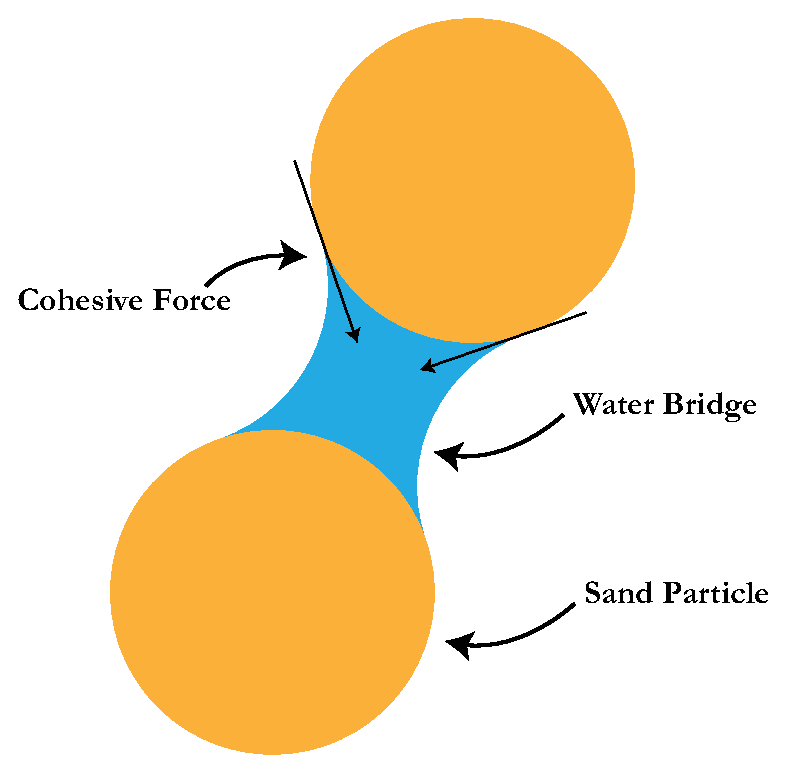
\includegraphics[width=0.5\linewidth]{water_bridge.eps}
    \caption{Water Bridge Between Sand Particle}
    \label{fig:water_bridge}
\end{figure}

\subsection{Our Work}
Normally people would sculpt their kingdom from a pile of tedious wet sand. To simplify the model and grasp main threads, we'll focus our research on this single, nondescriptive mound of wetted sand. In this article, we develop a method for determining the most long-lasting three dimensional shape for a tedious sand castle, which will be later referred to as \textit{sand castle foundation}.
\par
Our model addresses the problem of constructing a three dimensional structure by projection, which makes the construction of individual part of our model easy to implement. Firstly we determine the optimal \textit{side view} of our \textit{sand castle foundation} by analysing and extracting information from similar research on wet granular material\autocite{mitarai2006wet}. Then we construct the best \textit{top view} of the \textit{sand castle foundation} by constructing a \textbf{Cellular Automata}.

\paragraph{Side Slope Determination}
You've probably seen questions about the slope of a pile of dry sand in junior high school practice books. In our research, we address the problem about dry sand as a normal junior high student would. However, the analysis of wet sand requires some technique beyond low level physics. In our research, we establish this model using \textbf{Mohr-Coulomb Criterion}.

\paragraph{Top View Determination}
Our model analyses the impact of sea wave flow from a top view, or a \textit{slice} of the \textit{sand castle foundation}. Then we can combine the sliced impaction result together with the \textit{side slope} analysis to form a possible 3D object. Inside our model we construct a \textbf{Cellular Automata} since the shape of the sand slice edge isn't as obvious the side slope may be, that is, it's merely possible to construct continuous function on the shape.

\paragraph{Other Factors}
It's worth noting that the interaction between sand and sea wave is far a lot more complex than direct force impact or sand-to-water mixture proportion change. Some other factors include: gravity of sea water that submerge the sand underneath, influx of weaker sea wave and the gravity of water inside the wetted sand. During the assembly of two views, we'll address these other factors that may influence a \textit{sand castle foundation}'s life span.

\section{Assumptions \& Nomenclature}
\subsection{Assumptions}
Several assumptions are made in order to simplify our model.
\begin{itemize}
    \item [1)]
          The weather condition is suitable for sbuilding sand castles. Namely, no huge waves occur.
    \item [2)]
          The sand castle foundation is set where the maximum height of wave does not exceed a certain value, which we set as 0.2m for convenience, when the tide rises.
    \item [3)]
          Our optimization goal is to acquire the largest top size while minimizing the lost of sand. Intuitively, if the side of the foundation is built as a gentle slope, the possibility of collapsing will be drastically reduced. However, with a fixed volume of sand, such a foundation will not allow any sophisticated carving.
    \item [4)]
          Sand grains are regarded as tiny spheres. In our foundation, these grains are of the same size and are closely packed.
    \item [5)]
          The top of the foundation is a flat platform whose surface is horizontal.
    \item [6)]
          The side further from the sea has the same slope as the side facing the sea, as when waves recede, its 
\end{itemize}
\subsection{Nomenclature}
\begin{table}[H]
    \caption{States of Sand}
    \vspace{5pt}
    \centering
    \begin{tabular}{cl}
    	\hline
        Symbol     & Meaning                                                \\
        \hline
        $\tau$     & the shear stress on a plane                            \\
        $\tau_f$   & the shear stress on the failure plane                  \\
        $\mu$      & the internal friction coefficient                      \\
        $\sigma$   & the normal compressible stress on a plane              \\
        $\sigma_f$ & the normal compressible stree on the failure plane     \\
        $\rho$     & the density of sand                                    \\
        $\theta_c$ & the critical angle of a sandpile                       \\
        $D$        & the height from the top of the sand pile               \\
        $P$        & the pressure[]                                         \\
        $\Gamma$   & the surface tension of water                           \\
        $s_A$      & the adhesive stress                                    \\
        $f_A$      & the adhesive force                                     \\
        $V$        & the total amount of fluid present per particle contact \\
        $R$        & the radius of particle                                 \\
        $c_{ijk}(t)$ & the cell mixed with sand and water to form the sandcastle in time t \\
        $s_{ijk}(t)$ & the amount of sand in the cell in time t                            \\
        $w_{ijk}(t)$ & the amount of water in  $c_{ijk}$ in time t                         \\
        $p_{ijk}(t)$ & the proportion of sand-to-water mixture $c_{ijk}$ in time t         \\
        $S(t)$       & the amount of sand in the sandcastle	int time t                      \\
        $W(t)$       & the amount of water in the sandcastle in time t                     \\
        $P(t)$       & the average proportion of sand-to-water mixture $c_{ijk}$ in time t \\
        $F(t)$       & the erosion-Osmosis common effect of the sea water in time t        \\
        \hline
    \end{tabular}
    \label{bs2}
\end{table}

\section{Modeling Under Waves and Tides}
\par
The 3-dimensional shape constructing problem is divided into two sub-problems. We first establish the model using the \textbf{Mohr-Coulomb Criterion} to decide the shape of the slope, then construct another model with a modified version of \textbf{Cellular Automata} to determine the best shape viewed from the top.

\subsection{Shape of the Slope: Mohr-Coulomb Criterion}
We begin by determining the side shape of the sand castle foundation. Before Approaching the problem, we will briefly address the property of sand as a granular media.
\par
In our assumptions, sand particles are considered as identical tiny spheres. If we zoom in to observe a pile of wet sand, there are the so-called liquid bridges formed between sand particles.
\par
Various water contents produce different liquid bridge distributions, which will influence the properties of sand.

\begin{table}[H]
    \caption{States of Sand}
    \vspace{10pt}
    \centering
    \begin{tabular}{cccl}
        \hline
        Liquid Content   & State     & Description                                    & Schematic                  \\
        \hline
        No               & Dry       & No cohesive force exists                       & \begin{minipage}{0.5\textwidth}
            
\includegraphics[width=1.5cm, height=1.125cm]{s1.png}
        \end{minipage}  \\
        Small            & Pendular  & Liquid bridges start to form                   & \begin{minipage}{0.1\textwidth}
            
\includegraphics[width=1.5cm, height=1.125cm]{s2.png}
        \end{minipage} \\
        Middle           & Funicular & Liquid bridges and liquid-filled pores coexist & \begin{minipage}{0.1\textwidth}
            
\includegraphics[width=1.5cm, height=1.125cm]{s3.png}
        \end{minipage} \\
        Almost saturated & capillary & Almost all pores are filled with the liquid    & \begin{minipage}{0.1\textwidth}
            
\includegraphics[width=1.5cm, height=1.125cm]{s4.png}
        \end{minipage} \\
        More             & Slurry    & No cohesive force exists                       & \begin{minipage}{0.1\textwidth}
            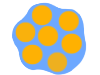
\includegraphics[width=1.5cm, height=1.125cm]{s5.png}
        \end{minipage} \\
        \hline
    \end{tabular}
    \label{bs2}
\end{table}
\par
When the wave gets into contact with the foundation, the surface area is in slurry state and there exists no cohesive interaction between the particles, which makes it very hard, if not impossible, to prevent sand loss in this process. Nevertheless, collapses after the wave resides can cause more harm to the foundation, which can be avoided by alternating the shape.
\par
When the wave gets into contact with the foundation, the surface area is in slurry state and there exists no cohesive interaction between the particles, which makes it very hard, if not impossible, to prevent sand loss. Nevertheless, collapses after the wave resides can cause more harm to the foundation, which can be avoided by alternating the shape.
\par
For dry sand, the failure criterion is given in terms of the shear stress $\tau$, the normal compressible stress $\sigma$ and the internal friction $\mu$ as
$$\tau > \mu\sigma$$
This is simply the friction formula with different notations. For wet sand, we consider a sandpile with a normal adhesive stress $s_A$ across every plane, in addition to the stress caused by weight. The equation(1) is then modified as
$$\tau > \mu(\sigma + s_A)$$
This is the so-called \textbf{Mohr-Coulumb criterion}. The stress resulting from the weight above the plane is shown in figure(2). Denote $\tau_f$ and $\mu_f$ as the shear stress and normal compressible stress at the failure plane, it is obvious from the schematic that they can be written as
$$\tau_f = \rho gDsin\theta_c \qquad and \qquad \sigma_f = \rho gDcos\theta_c$$
where $\theta_c$ is the critical angle, $D$ is the height of the sandpile and $\rho$ is the density of sand. Therefore, combine the equations above, to solve for $\theta_c$ is to solve the equation
$$\mu = tan\theta_c(D)\bigg(1 + \frac{s_A}{\rho gDcos\theta_c(D)}\bigg)$$
\par
The only unknown factor is $s_A$, the adhesive stress across the plane. According to (Thomas C.H and Alex J.L -fix later)'s study, the value of $s_A$ is determined by water content and there are three regimes as a function of the added-fluid volume. We now focus only on the state where the water content is close to saturation.
\par
In this case, with water serves as lubricate, it makes sense to model sand particles as frictionless spheres. The pressure difference is then given by []
$$P = -\frac{\Gamma}{\sqrt{V/2\pi R}}$$
where $\Gamma$ is the surface tension of the fluid, V is the total amount of fluid present per particle contact, and R the radius of the particle. According to the study of [fix later], the adhesive force in this state is given by
$$f_A = 2\pi \Gamma R$$
Note that (with certain conditions like distance between grains remains constant)the term $V$ which denotes the volume of liquid per particle does not appear in equation(6).
\par
We now focus on obtaining the value of $s_A$ via $f_A$, whose value can be calculated with the equation above. Assume our foundation contains sand particles that are closely packed. In such a structure, we have $\phi_V = \sqrt(2)/6$, where $\phi_V$ stands for volume fraction which is defined as ratio of the volume of particles to the total volume. The average number of contacts per unit area will be $(3\phi_V/\pi R^2)$. With $f_A$ representing cohesive force of a single liquid bridge, we can then write
$$ s_A = \frac{f_A}{\sqrt{2}R^2}$$
Substitute the above result into Eq.(), we obtain the result
$$ tan\theta_c = \mu + \frac{\sqrt{2}\pi\mu\Gamma}{R\rho gD}sec[tan^{-1}(\mu)] $$

\subsection{Top View Shape}
\par
We used a modified version of\textbf{ cellular automata} to simulate the impact of tides and waves. There are several factors that are taken into consideration:
\par
\begin{itemize}
    \item [1)]
          ...
    \item [2)]
          ...
    \item [3)]
          ...
\end{itemize}

\begin{figure}[H]
    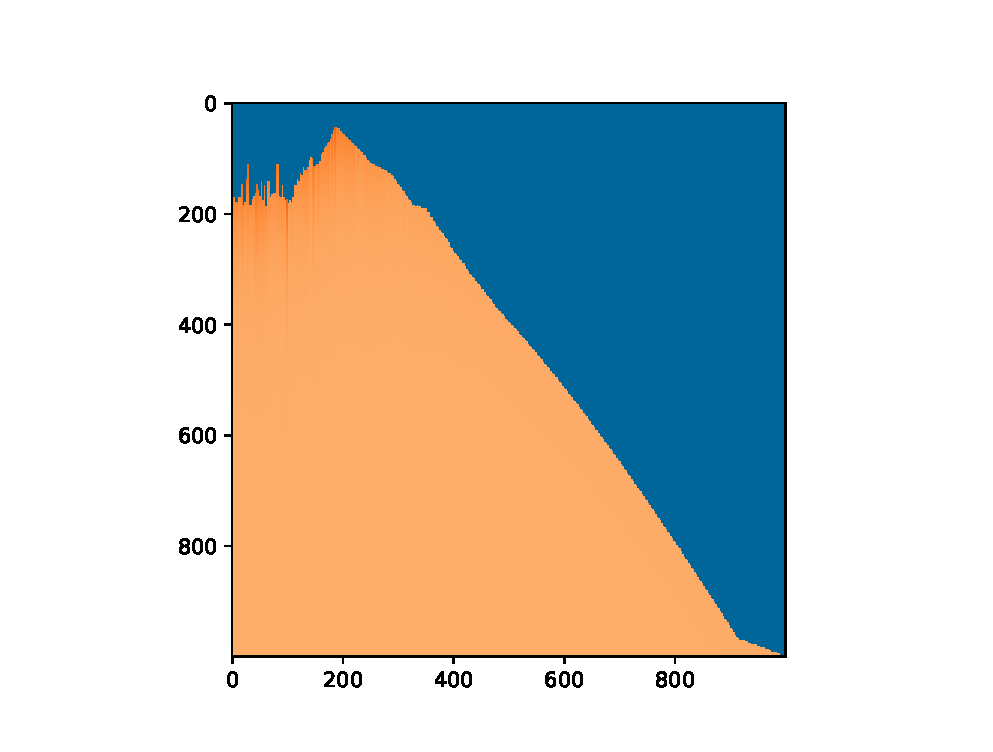
\includegraphics[width=\linewidth]{Figure_1.eps}
    \caption{A Windows Terminal.}
    \label{fig:Terminal}
\end{figure}
\textcolor{cyan}{This is a test figure. Remember to delete me.}
\begin{figure}[H]
    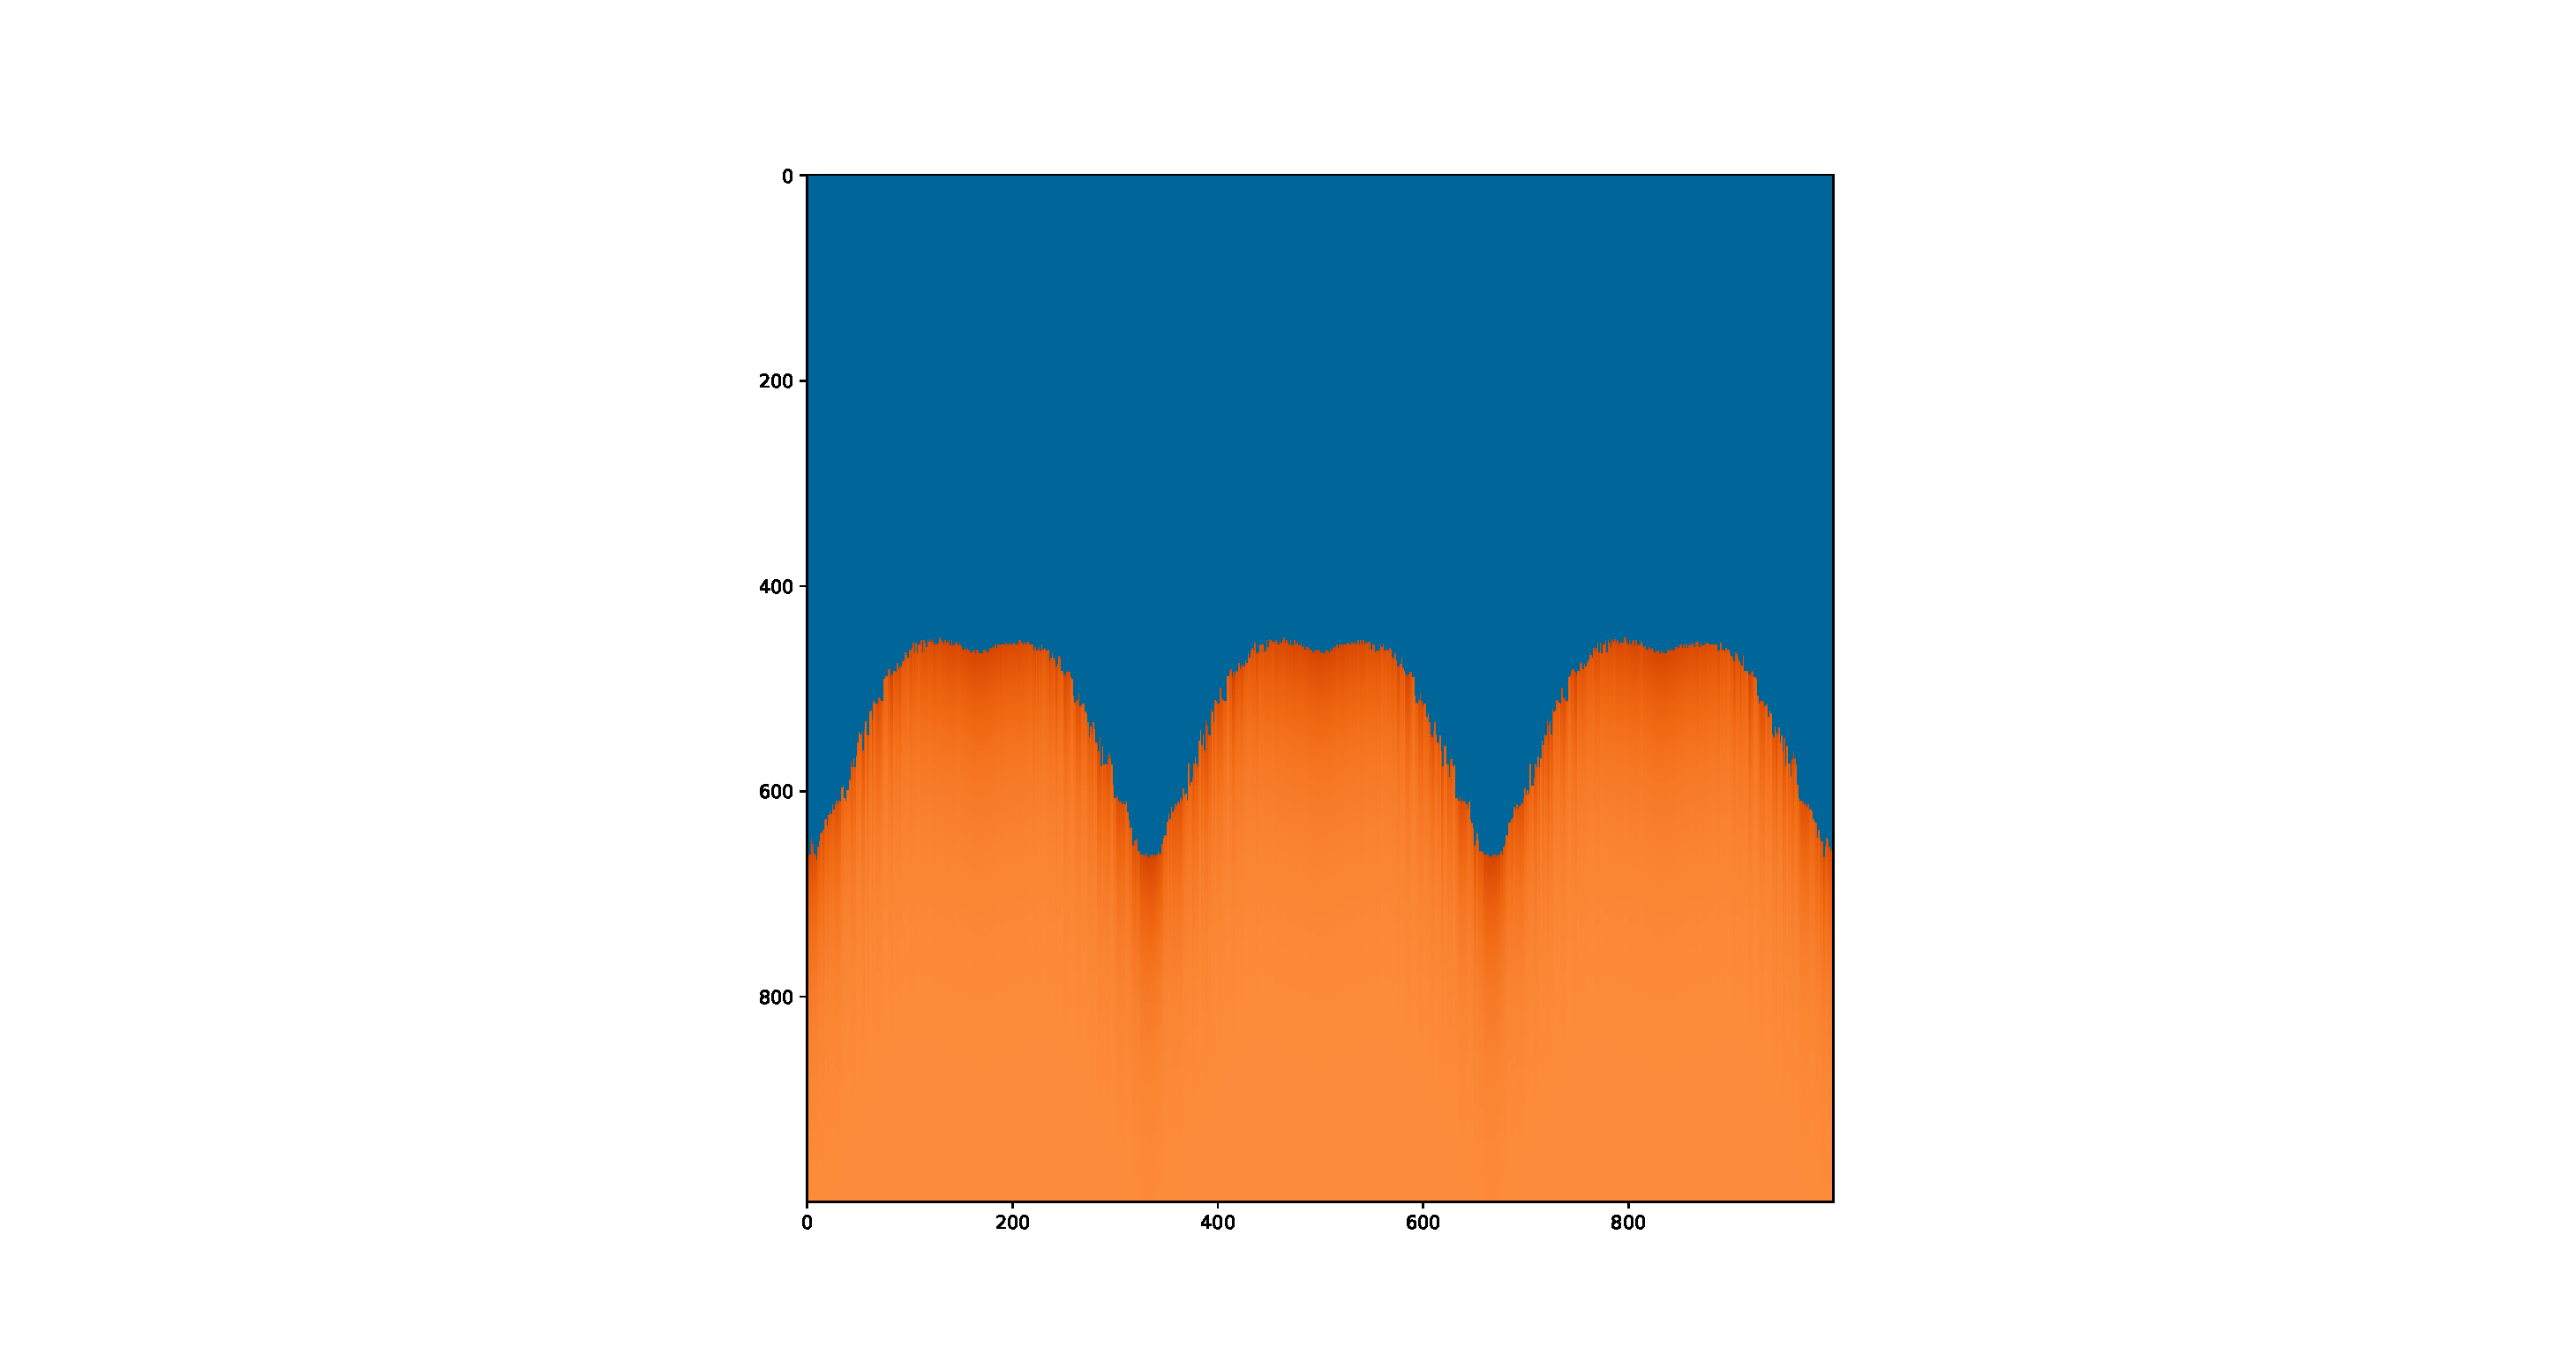
\includegraphics[width=\linewidth]{Figure_2.eps}
    \caption{A Windows Terminal.}
    \label{fig:Terminal}
\end{figure}

\subsection{Calculate \& Simulate Results}
Briefly review the equation derived in section 3.1
$$tan\theta_c = \mu + \frac{\sqrt{2}\pi\mu\Gamma}{R\rho gD}sec[tan^{-1}(\mu)]$$
To solve for the best shape of the slope, the necessary information about sand is listed below
\begin{table}[H]
    \caption{States of Sand}
    \vspace{10pt}
    \centering
    \begin{tabular}{ccc} 
        \hline
        Physical Quantities & Values    & Units    \\
        \hline
        $\Gamma$            & 72.8      & $mN/m$   \\
        $\mu$               & 0.55~0.60 & -        \\
        $\rho$              & 1631      & $kg/m^3$ \\
        $R$                 & 0.05~2    & $mm$     \\
        $g$                 & 9.81      & $m/s^2$  \\
        \hline
    \end{tabular}
    \label{bs2}
\end{table}
\par
It is not sensible to embark on a trip to the beach on a stormy day, so we assume that the near-shore wave is gentle, with its height not exceeding 20cm, or $D \in [0, 20](unit:cm)$.
We adopt $\Gamma = 72.8mN/m$, $\mu = 0.55$, $\rho = 1631kg/m^3$, $R = 2mm$ and $g = 9.81m/s^2$. 
\begin{figure}[H]
	\centering
	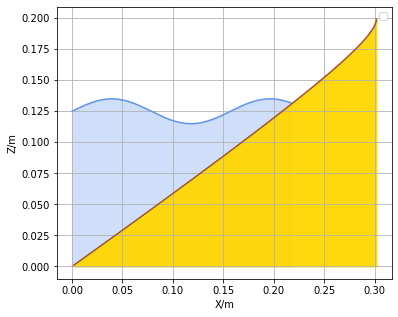
\includegraphics[width=8cm, height = 6.67cm]{sand5.png}
	\caption{A Windows Terminal.}
	\label{the shape of the slope}
\end{figure}
\begin{table}[H]
	\caption{States of Sand}
	\vspace{10pt}
	\centering
	\begin{tabular}{ccc} 
		\hline
		Height(m) & Slope     \\
		\hline
		0.02            & 0.58     \\
		0.04            & 0.58  \\
		0.06            & 0.59      \\
		0.08            & 0.60    \\
		0.10            & 0.60      \\
		0.12			& 0.61 \\
		0.14  			& 0.63\\
		0.16			& 0.66\\
		0.18			& 0.71\\
		0.20            & 0.88 \\
		\hline
	\end{tabular}
	\label{bs2}
\end{table}
\section{Modeling Under Rain}
\subsection{Model Adaptations}
Rain differs from waves and sands in the following aspects: its continuity, and its quantity. So we modify our Cellular Automata model to adapt to the new conditions.
\paragraph{Adaptations}
\begin{itemize}
    \item [1)]
          In our previous model, wave is modeled as discrete motions.
    \item [2)]
          Rainwater can wet our model in a relatively short time.
    \item [3)]

\end{itemize}
\subsection{Shape Alteration}
As a result, our model is not the most preferable option under the rain. Shape alterations have to be made if we want our sand castle foundation to last longer.
\section{Determine the Best Sand-to-water Proportion}
\subsection{Assumptions \& Nomenclature}
\textcolor{cyan}{ADD A CURVE FIGURE HERE, DRAWING!}
\par
As we mentioned above, the adhesive stress across the plane ( $s_A$ ) is determined by water content. Consequently, we will find out how the cohesion in wet granular materials varies with different amount of liquid based on liquid bridge model to find an optimal sand-to-water mixture proportion.
\par
There are five differing degrees of wetting in granular matter. As dry grains and slurry have no cohesion between particles, we just consider three other conditions. According to [2], we can see that the slope for low and large liquid content is much larger than that for intermediate liquid content. That is: the suction changes sharply as these three states transform each other. Consequently,we should keep the proportion of water to sand in steady for a long time, which means try to avoid transformation between three states.
\par
we initially wish to create a three dimensional matrix to represent the situation. We still consider that the sandcastle $C$ consists of cells mixed with sand and water. Then It's easy to Calculate each cell’s sand-to-water mixture proportion from the amount of sand and water.
\textcolor{cyan}{ADD TWO CELLULAR FIGURES HERE, DRAWING!}
\subsection{Assumptions}
\begin{itemize}
    \item [1)]
          waves and tides erode the sandcastle in a very short time, which means that the we can neglect Osmosis occurred during erosion.
    \item [2)]
          After eroded, the liquid left on sandcastle has ample time to penetrate.
    \item [3)]
          The evaporation of liquid is neglected.
\end{itemize}
\subsection{Review on Nomenclature}
\begin{table}[H]
    \caption{Notation Table}
    \vspace{10pt}
    \centering
    \begin{tabular}{ |l| p{5cm}| } 
        \hline
        symble       & meaning                                                             \\
        \hline
        $c_{ijk}(t)$ & the cell mixed with sand and water to form the sandcastle in time t \\
        $s_{ijk}(t)$ & the amount of sand in the cell in time t                            \\
        $w_{ijk}(t)$ & the amount of water in  $c_{ijk}$ in time t                         \\
        $p_{ijk}(t)$ & the proportion of sand-to-water mixture $c_{ijk}$ in time t         \\
        $S(t)$       & the amount of sand in the sandcastle	int time t                      \\
        $W(t)$       & the amount of water in the sandcastle in time t                     \\
        $P(t)$       & the average proportion of sand-to-water mixture $c_{ijk}$ in time t \\
        $F(t)$       & the erosion-Osmosis common effect of the sea water in time t        \\
        \hline
    \end{tabular}
    \label{bs1}
\end{table}
\subsection{Model}
We define the expression when we just finish build the sandcastle.
$$  P(t_0) = \frac{S(t_0)}{W(t_0)} = \frac{\sum_{i,j,k}s_{ijk}(t_0)}{\sum_{i,j,k}w_{ijk}(t_0)} = p_{ijk}(t_0) $$
\par
To evaluate the existence of the sandcastle, we define that a cell is completely eroded by tides and waves as follow:
$$  p_{ijk}(t) = \frac{s_{ijk}(t)}{w_{ijk}(t)} \leq p_{erode} $$
\par
And we define that the sandcastle is completely eroded as:
$$  P(t) = \frac{\sum_{i,j,k}s_{ijk}(t_0)}{\sum_{i,j,k}w_{ijk}(t_0)} \leq P_{erode} $$
\par
where $P_{erode}$ refers to proportion that Funicular transforms to capillary state. Then we define the flow equation during erosion as follow:
$$	E=
    \begin{cases}
        F & \text{the cell is being eroded by sea} \\
        0 & \text{else}
    \end{cases}
$$
\par
As erosion occurs for a split second, we could just neglect the permeation to simplify our analysis. To obtain a probability model to evaluate the sand taken by waves, we need to acquire further understanding about the flow liquid. Here we use Navier-Stokes equations to describe the motion of viscous fluid substances.
$$
    x \rho(\frac{\partial \upsilon}{\partial t} + \upsilon \cdot \nabla \upsilon) = -\nabla p + \nabla \cdot(\mu(\nabla \upsilon+(\nabla \upsilon)^T)-\frac{2}{3}\mu(\nabla \upsilon)I)+F\\\frac{\partial \rho}{\partial t}+\rho\nabla\cdot\vec{\upsilon}=0(continuity \ equations)
$$
\par
After eroded we should find the cell completely eroded by tides and waves. Then by reference to Darcy's law and Huygens–Fresnel principle, We consider water permeating the sandcastle as follow:
$$
    \upsilon=\frac{kA(p_b-p_a)}{\mu L}=\frac{kL(\Delta P)}{\mu}
$$
\par
where $k$ is the hydraulic permeability of sea water, $L$ is the length of one side of the cell, $\mu$ is the viscosity of sea water, $\Delta$ is the pressure differential between the two sides of the cell.As we assume that the sea water left on the surface of the sandcastle can totally penetrate. Then we could get for each cycle:
$$
    L (k,t,\mu,\rho,\upsilon,p)=\sum_{c_{ijk}\in C}\sum_{i-1}^{i+1}\sum_{j-1}^{j+1}\sum_{k-1}^{k+1}{p_{mnp}\cdot E}(m,n,p \neq i,j,k)(P(t) <P_{limit})\\
    (\upsilon \cdot \nabla \upsilon)+(\mu \cdot \nabla \mu)+(\rho \cdot \nabla \rho) = Constant
$$
\par
Then We need to find out the longest time when the above constraints are met and the sandcastle exists.

\section{Other Tricks to Make Our Sand Castle Last Longer}
\subsection{Build a Moat}
Building a moat can help our sand castle foundation to survive the rising tide. With the help of a moat, waves recede before they can hit the foundation, which significantly prolongs the life of the foundation.
\subsection{Make It Compact}
There are two advantages of making a compact foundation. 
\paragraph{More Contact Points}
In section 3.1, we assumed that sand particles are closely packed. 
\paragraph{Fewer Cracks}
\subsection{Further From the Shore}
According to our analysis in section 5, the optimal sand-to-water proportion is 1\%.
(This is not possible if the castle can be reached by wave...)
\subsection{Finer Sand}
Finer sand is a bonus because by constructing our sand castle foundation using finer sand, the foundation has a greater critical angle. That is because the radius of particles $R$ which is a part of the denominator decreases and (enlarge?not the proper word) the value of $tan\theta_c$.
\subsection{Special Material}
\paragraph{Glue}
Sand sculptures seen in exhibitions or competitions have their surfaces covered with special glue. The glue is mainly used to protect the sand sculpture from drying out or crumbling if the waves do not wash it away first, but it can also keep water out. In our model where the greatest enemy of the foundation is not collapses but erosion, such glue will help maintain the shape of the foundation.
\paragraph{Mixture}
Concrete, a material that everyone is familiar with, has sand as its ingredient.
\subsection{Less Salty Water}
Choosing a beach near a less salty ocean may contribute to building a more concrete sand castle. This is because fresh water has a higher value of surface tension which appears in the numerator of the term $\frac{\sqrt{2}\pi\mu\Gamma}{R\rho gD}$. Thus Red Sea is not a perfect spot, but the Baltic Sea(poor English. better expression needed.)(footnote needed)
Finer sand is a bonus because by constructing our sand castle foundation using it, the foundation has a greater critical angle. That is because the term $R$, which is a part of the denominator, decreases and (enlarge?not the proper word) the value of $tan\theta_c$.
\subsection{Special Material}
\paragraph{Glue}
Sand sculptures seen in exhibitions or competitions have their surfaces covered with special glue. The glue is mainly used protect the sand sculpture from drying out or crumbling if the waves do not wash it away first, but it also keeps water out. In our model where the greatest enemy of the foundation is not collapses but erosion, such glue will help maintain the shape of the foundation.
\paragraph{Mixture}
Concrete, a material that everyone is familiar with, has sand as its ingredient.

\section{Sensitivity Analysis}
\subsection{Model Under Waves and Tides}
\paragraph{Side View Shape}
\par
There are multiple factors that may affect our side view shape model. We consider four of them: the internal friction coefficient $\mu$, radius of the sand particles $R$, density of sand $\rho$ and total height of the sand castle foundation $D$.
\par
Friction coefficient of sand varies by the amount of liquid in the system, the size of sand grains and other possible factors. Typically, this value ranges from 0.55-0.60. In figure[x.a], we test the effect of different friction coefficient ranging from 0.48 to 0.60. The curves with lighter colors, as illustrated in the figure, represent higher coefficients while those with darker colors represent lower coefficients.
\par
Figure[x.b] shows how the side view shape is influenced by radius of the sand particles, which varies between 0.5 to 2.0 milimeters. Curves with lighter colors represent small particle radiuses and those with darker colors represent greater radiuses.
\par
The effect of density is illstrated in Figure[x,c], which is not obvious compared with the former two factors.
\begin{table}[H]
    \caption{}
    \vspace{10pt}
    \centering
    \begin{tabular}{p{6.5cm}p{6.5cm}} \\ 
        \begin{minipage}{0.5\textwidth}
            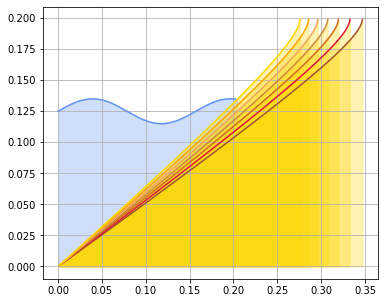
\includegraphics[width=6cm, height=5cm]{sand1.png}
        \end{minipage}
         & \begin{minipage}{0.5\textwidth}
            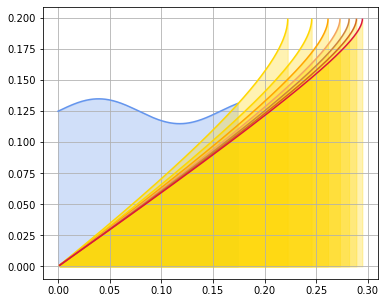
\includegraphics[width=6cm, height=5cm]{sand2.png}
        \end{minipage} \\
        \begin{minipage}{0.5\textwidth}
            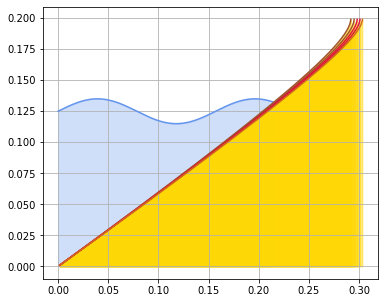
\includegraphics[width=6cm, height=5cm]{sand3.png}
        \end{minipage}
         & \begin{minipage}{0.5\textwidth}
            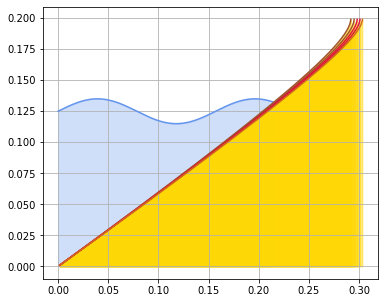
\includegraphics[width=6cm, height=5cm]{sand3.png}
        \end{minipage} \\
    \end{tabular}
    \label{bs2}
\end{table}
\paragraph{Top View Shape}
DenDen dl has done a lot of parameter adjusting jobs...those are exactly what we need here.
\subsection{Model Under Rain}
Not now. Wait for tomorrow or something.


\section{Strengths and Weaknesses}
\subsection{Strengths}
Just like any other model, the one presented above has its Strengths and Weaknesses. Some major points are listed below.
\begin{itemize}
    \item [1)]
	    \textbf{Flexibiliry and extendibility}\\
	    The use of Cellular Automata enables our model to predict erosion of any possible shape. For those who are not satisfied with a dull, oval-like shape, our model can assist them in finding more interesting shapes with relatively small losses.
    \item [2)]
	    \textbf{Taking Future into Consideration}\\
	    Cellular Automata can simulate the whole life-cycle of the sand castle foundation. Thus we are judging a shape by not only its current performance, but also how it performs after its shape has been changed.
    \item [3)]
	    \textbf{Taking into Consideration the Height of Waves}\\
	    Due to tidal effects, the height of the waves is not a constant. From the analysis in section 3.1, the shape identified can resist waves from t
\end{itemize}
\subsection{Weaknesses}
\begin{itemize}
    \item [1)]
    \textbf{Not accurate enough}\\
    Our model in section 3.1 is actually an approximation of reality, as in capillary state, the amount of water is very close to saturation, which means liquid bridges only play a minor role in stabilizing the sand castle foundation. Even though in Funicular state, where the cohesive stress $s_A$ increases monotonically with water content for most of the time, the two states differ in properties and will bring loss to our model.
    \item [2)]
    \textbf{Simplistic Assumptions}\\
    To acquire computability, we simplify the effect of waves to be wetting and hitting the surface. Nevertheless, the flow direction is also of vital significance, about which we fail to fully consider.
    
\end{itemize}

\section{Future Developments}
\par 
We can 
%\textcolor{cyan}{This is a test figure. Remember to delete me.}



%This is some example text\footnote{\label{myfootnote}Hello footnote}.

%I'm referring to footnote \ref{myfootnote}.


\newpage
\begin{appendix}
    \listoffigures
    \listoftables
    \listoflistings
    % \bibliographystyle{ieeetr}
    \printbibliography
\end{appendix}
\end{document}
